\documentclass[oneside]{report}
\usepackage[utf8]{inputenc}
% \usepackage[vietnamese]{babel}
\usepackage[T5]{fontenc}
\usepackage{graphicx}
\usepackage{nameref}
\usepackage{multicol}
\usepackage[vietnamese, main=english]{babel}

% set font, font size and spacing
\usepackage{times}
\usepackage{scrextend}
\changefontsizes{13pt}
\renewcommand{\baselinestretch}{1.3}

% section spacing
\usepackage{titlesec}
\titlespacing*{\section}{0pt}{0.5\baselineskip}{0.2\baselineskip}
\titlespacing*{\subsection}{0pt}{0.4\baselineskip}{0.2\baselineskip}

% setup page layout
\usepackage[a4paper,left=30mm,top=20mm,bottom=25mm,right=20mm,]{geometry}

% Acronyms Auto
\usepackage[nopostdot,toc,acronym,nomain,nonumberlist]{glossaries}
\makeglossaries
\setacronymstyle{long-short}
\loadglsentries[acronym]{FrontMatter/Acronyms}
\setlength{\glsdescwidth}{0.7\linewidth}

% % prevent text overflow
% \usepackage{babel}
% \newcommand\fh{\babelhyphen{hard}}

% Change indent
% \usepackage{indentfirst} % indent also after section titles
\setlength{\parindent}{1cm}
\usepackage{enumitem}
\setlist{leftmargin=1cm}

% paragraph spacing
\setlength{\parskip}{0.5em}

% Change enumerate label
\usepackage{enumitem}

% Page numbering at the center top of page
% \usepackage{fancyhdr} % Custom headers and footers
% \pagestyle{fancyplain} % Makes all pages in the document conform to the custom headers and footers
% \fancyhead[L]{}% Empty left header
% \fancyhead[C]{\thepage} % Page numbering for center header  
% \fancyhead[R]{}% Empty right header
% \fancyfoot[L]{}% Empty left footer
% \fancyfoot[C]{}% Empty center footer
% \fancyfoot[R]{}% Empty left footer

% natbib
% if use natbib, please comment out the cite
\usepackage[sort,numbers]{natbib}
% Citation
% \usepackage{cite}

% Math equation
\usepackage{amssymb}
\usepackage{amsmath}

% Table
\usepackage{multirow}
\usepackage{longtable}
\usepackage{bigstrut}

% Cover
\usepackage{pdfpages}

% Subfigure
\usepackage{caption}
\usepackage{subcaption}

% pstricks fig
\usepackage{epsfig}

% Table of Contents
\usepackage[hidelinks]{hyperref}
% Uncomment if you want leading dot for chapter
\usepackage{tocloft}
\renewcommand{\cftpartleader}{\cftdotfill{\cftdotsep}} % for parts
\renewcommand{\cftchapleader}{\cftdotfill{\cftdotsep}} % for chapters

% table fixed width column
\usepackage{array}
\newcolumntype{L}[1]{>{\raggedright\let\newline\\\arraybackslash\hspace{0pt}}m{#1}}
\newcolumntype{C}[1]{>{\centering\let\newline\\\arraybackslash\hspace{0pt}}m{#1}}
\newcolumntype{R}[1]{>{\raggedleft\let\newline\\\arraybackslash\hspace{0pt}}m{#1}}

\hyphenation{Nan-yang}

\title{GRAPH ATTENTION NETWORKS}
\author{Đoàn Văn Nguyên, Nguyễn Đức Trọng, Nguyễn Trần Đạt}
\date{February 2022}

\begin{document}

% thử tiếng việt
%---------------------------------------------
% Front Matter
%---------------------------------------------

\includepdf[pages=-]{FrontMatter/cover.pdf}
\pagenumbering{roman}
\setcounter{page}{3}
\chapter*{Abstract}
\addcontentsline{toc}{chapter}{Abstract}

Chúng tôi giới thiệu Graph Attention Network (GAT), mô hình mạng nơ-ron mới hoạt động trên dữ liệu dạng đồ thị, sử dụng các lớp tự quan tâm đã đặt mặt nạ để cải thiện những nhược điểm của các phương pháp trước đó dựa trên hỗn hợp đồ thị hoặc các ước lượng của chúng. Bằng cách xếp lớp trong đó các nút có thể quan tâm đến các đặc trưng của lân cận, chúng ta cho phép (ẩn dụ) chỉ định các trọng số khác nhau cho các nút trong một lân cận, mà không cần bất kỳ hoạt động ma trận chi phí (như đảo ngược) hoặc phụ thuộc vào việc biết cấu trúc đồ thị trước.
Theo cách này, chúng tôi giải quyết một số vấn đề chính của các mạng nơ-ron đồ thị dựa trên tần số cùng lúc, và làm cho mô hình của chúng tôi dễ dàng áp dụng cho cả vấn đề dẫn chứng và dẫn điểm. Mô hình GAT của chúng tôi đã cho kết quả ??? trên bốn mô hình kiểm thử transductive và inductive: các tập dữ liệu Cora, Citeseer và Pubmed, cùng với tập dữ liệu tương tác protein-protein (ở đây, test graph bị ẩn trong quá trình học máy).


\vspace{8pt}
\noindent \textit{\textbf{Keywords}: Graph Attention Networks(GAT), transductive, Vietnamese multi-aspect dataset.}


\chapter*{Acknowledgements}
\addcontentsline{toc}{chapter}{Acknowledgements}

Lời đầu tiên, chúng em xin cảm ơn Cô Nguyễn Thị Cẩm Vân và các thầy cô trong lab  Data Science and Knowledge Technology Laboratory at University of Engineering and Technology. Các thầy cô đã luôn giúp đỡ và hướng dẫn chúng em viết ra bài báo này.


% We also want to acknowledge my co-supervisor Assoc.Prof Chng Eng Siong from Nanyang Technological University, Singapore for offering me the internship opportunities at NTU, Singapore and leading me working on diverse exciting projects.

% Furthermore, I am very grateful to my external advisor MSc. Le Hoang Quynh, for insightful comments both in my work and in this thesis, for her support, and for many motivating discussions.

% In addition, we have been very privileged to get to know and to collaborate with many other great collaborators.
% I would like to thank BSc. Nguyen Minh Trang and BSc. Nguyen Duc Canh for inspiring discussion, and for all the fun we have had over the last two years.
% I thank to MSc. Ho Thi Nga and MSc. Vu Thi Ly for continuous support during the time in Singapore.

% Finally, I must express my very profound gratitude to my family for providing me with unfailing support and continuous encouragement throughout my years of study and through the process of researching and writing this thesis.
% This accomplishment would not have been possible without them.

Đồng thời em cũng xin cảm ơn khoa Công nghệ thông tin - Trường Đại học Công nghệ đã tạo điều kiện để cho chúng em có được trải nghiệm thực tế trong môi trường nghiên cứu khoa học và tiếp thu nhiều kiến thức bổ ích.
\chapter*{Declaration}
\addcontentsline{toc}{chapter}{Declaration}
We declare that our work has been composed by ourselves and that the work has not be submitted for any other degree or professional qualification.
We confirm that the work submitted is ou own, except where work which has formed part of jointly-authored publications has been included.
Our contribution and those of the other authors to this work have been explicitly indicated below.
We confirm that appropriate credit has been given within this article where reference has been made to the work of others.

% The model presented in Chapter~\ref{chap:model} and the results presented in Chapter~\ref{chap:result} was previously published in the Proceedings of ACIIDS 2019 as \textit{``Improving Semantic Relation Extraction System with Compositional Dependency Unit on Enriched Shortest Dependency Path''} and NAACL-HTL 2019 as \textit{``A Richer-but-Smarter Shortest Dependency Path with Attentive Augmentation for Relation Extraction''} by myself et al.
% This study was conceived by all of the authors.
% I carried out the main idea(s) and implemented all the model(s) and material(s).

We certify that, to the best of our knowledge, our article does not infringe upon anyone’s copyright nor violate any proprietary rights and that any ideas, techniques, quotations, or any other material from the work of other people included in my thesis, published or otherwise, are fully acknowledged in accordance with the standard referencing practices.
Furthermore, to the extent that we have included copyrighted material, we certify that we have obtained a written permission from the copyright owner(s) to include such material(s) in our work and have fully authorship to improve these materials.

\begin{table}[h]
\begin{tabular}{p{0.7\textwidth}c}
 & Student group \\
 &              \\
 &              \\
 &              \\
 & \textbf{Le Thi Phuong}\\
 & \textbf{Le Minh Binh}\\
 & \textbf{Tran Khanh Hung}\\
 & \textbf{Bui Khanh Huyen}
\end{tabular}
\end{table}

% Show ToC and change title to Table of Contents
\setcounter{secnumdepth}{3}
\renewcommand{\contentsname}{Table of Contents}
\addcontentsline{toc}{chapter}{Table of Contents}
\tableofcontents

% Show Acronyms and add it to ToC
\printglossary[title={Acronyms},type=acronym,style=long]
\clearpage




%--------------------------------------------- 
% Main content
%---------------------------------------------
\pagenumbering{arabic}
\setcounter{page}{1}
\chapter{Giới thiệu}
\label{chap:Giới thiệu}

% -------------------------------------------------------------------
% Motivation
% -------------------------------------------------------------------

Mạng Nơ-ron Tích Chập (Convolutional Neural Networks - CNN) hiện đang được áp dụng để giải các bài toán phân loại hình ảnh (He et al., 2016), phân vùng ngữ nghĩa ảnh (Jegou et al., 2017) hoặc dịch máy (Gehring et al., 2016), trong đó dữ liệu nền được biểu diễn dưới cấu trúc giống mạng lưới. Các mô hình này tái sử dụng hiệu quả các bộ lọc cục bộ, với các tham số học, bằng cách áp dụng chúng cho tất cả các vị trí đầu vào.

Tuy nhiên, nhiều tác vụ có liên quan đến dữ liệu không thể biểu diễn dưới dạng mạng lưới dưới dạng bất quy tắc. Bản dựng hình 3D, mạng xã hội, mạng viễn thông, mạng sinh học hoặc mạng kết nối não bộ là các ví dụ điển hình. Những loại dữ liệu này thường được biểu diễn dưới dạng đồ thị.

Trong lĩnh vực công nghệ thông tin, đã có một số nghiên cứu về việc mở rộng mạng nơ-ron để xử lý các đồ thị . Các nghiên cứu ban đầu sử dụng mạng nơ–ron đệ quy để xử lý dữ liệu được biểu diễn dưới dạng đồ thị đường vòng được định hướng (Frasconi et al., 1998; Sperduti \& Starita, 1997). Mạng Nơ-ron Đồ Thị (Graph Neural Network - GNN) được giới thiệu trong Gori et al. (2005) và Scarselli et al. (2009) là một mô hình chuẩn hóa của mạng nơ-ron đệ quy có thể trực tiếp xử lý các loại đồ thị bao quát hơn, ví dụ như đồ thị có chu trình, có hướng và không hướng. GNN bao gồm một quá trình lặp đi lặp lại, truyền trạng thái của nút cho đến khi đạt đối tượng; sau đó là một mạng nơ-ron, tạo ra một kết quả cho mỗi nút dựa trên trạng thái của nó. Ý tưởng này đã được Li et al. (2016) thừa hưởng và cải tiến bằng cách sử dụng đơn vị gated recurrent (Cho et al., 2014) trong bước truyền.

Tuy nhiên, việc mở rộng bộ lọc tổng quát cho không gian đồ thị đang càng ngày càng được quan tâm. Những tiến bộ theo hướng này thường được phân loại thành phương pháp quang phổ và phương pháp phi quang phổ. 

Một mặt, các phương pháp quang phổ hoạt động dựa trên một biểu diễn quang phổ của đồ thị và đã được áp dụng thành công trong bài toán phân loại nút. Trong Bruna et al. (2014), phép tích chập được xác định trong tầng Fourier bằng cách tính phân tích độ riêng của ma trận Laplacian của đồ thị, dẫn đến việc tính toán có thể nặng và bộ lọc không quang phổ tọa độ. Những vấn đề này đã được giải quyết bởi các công trình sau. Henaff et al. (2015) đã giới thiệu một tham số hóa của bộ lọc quang phổ với các hệ số mượt để làm cho chúng có tọa độ quang phổ. Sau này, Defferrard et al. (2016) đề xuất sử dụng phép mở rộng Chebyshev của ma trận Laplacian để ước lượng bộ lọc, loại bỏ việc tính toán các vector riêng của Laplacian và cho ra các bộ lọc có tính địa lý, Kipf \& Welling (2017) đã đơn giản hoá phương pháp trước bằng cách hạn chế bộ lọc hoạt động trong một vùng lân cận xung quanh mỗi nút. Tuy nhiên, trong tất cả các phương pháp đồng bộ hoá tần số trên, các bộ lọc được học phụ thuộc vào cơ sở vector riêng của Laplacian, điều này phụ thuộc vào cấu trúc đồ thị. Do đó, một mô hình được huấn luyện trên một cấu trúc cụ thể không thể được áp dụng trực tiếp cho một đồ thị với cấu trúc khác.

Mặt khác, các phương pháp phi quang phổ (Duvenaud et al., 2015; Atwood \& Towsley,2016; Hamilton et al., 2017) xác định việc tích chập trực tiếp trên đồ thị, hoạt động trên nhóm các đỉnh gần về vị trí. Một trong những thách thức của các phương pháp này là xác định một toán tử hoạt động với các lân cận có kích thước khác nhau và giữ thuộc tính chia sẻ trọng lượng của CNN. Trong một số trường hợp, điều này yêu cầu học một ma trận trọng lượng cụ thể cho mỗi bậc đỉnh (Duvenaud et al., 2015), sử dụng các lũy thừa của ma trận chuyển đổi để xác định lân cận và học trọng lượng cho mỗi kênh đầu vào và bậc lân cận (Atwood \& Towsley, 2016), hoặc trích xuất và chuẩn hóa các lân cận chứa số lượng cố định của đỉnh (Niepert et al., 2016). Monti et al. (2016) đã trình bày mô hình tổ hợp CNN (MoNet), một phương pháp vị trí cho phép tổng quát hóa kiến trúc CNN sang đồ thị. Gần đây, Hamilton et al. (2017) đã giới thiệu GraphSAGE, Một phương pháp tính biểu diễn của nút theo cách tuân theo. Kỹ thuật này hoạt động bằng cách mẫu một khu vực cố định kích thước của mỗi nút, sau đó thực hiện một trọng tải chung cho nó (như là trung bình của tất cả các vectơ đặc trưng của hàng xóm được mẫu, hoặc kết quả của việc cho chúng qua mạng nơ-ron tần suất). Phương pháp này đã cho kết quả tuyệt vời trên nhiều tiêu chuẩn thu hồi lớn.


% Attention Mechanism - dịch chuối vl

Cơ chế tập trung đã trở thành gần như một tiêu chuẩn trong nhiều tác vụ dựa trên chuỗi (Bahdanau et al., 2015; Gehring et al., 2016). Một trong những điểm mạnh của các mạng tập trung là xử lý với dữ liệu đầu vào có kích thước biến đổi, tập trung vào các phần quan trọng nhất của đầu vào để tính toán. Khi sử dụng mạng tập trung để tính toán một biểu diễn của một chuỗi, nó thường được gọi là tập trung tự hoặc tập trung trong. Cùng với mạng nơ-ron lặp lại (RNNs) hoặc tích chập, tập trung tự đã chứng minh là hữu ích cho các tác vụ như đọc máy (Cheng et al., 2016) và học biểu diễn câu (Lin et al., 2017). Tuy nhiên, Vaswani et al. (2017) cho thấy rằng tập trung tự không chỉ có thể cải thiện một phương pháp dựa trên RNNs hoặc tích chập, mà còn đủ để xây dựng một mô hình mạnh mẽ nhận được hiệu năng tiên tiến nhất trong tác vụ dịch máy.

Lấy cảm hứng từ công trình nghiên cứu trên, chúng tôi giới thiệu một kiến trúc dựa trên chú ý để thực hiện phân loại nút của dữ liệu cấu trúc đồ thị. Ý tưởng là tính toán biểu diễn ẩn của mỗi nút trong đồ thị, bằng cách chú ý trên các nút lân cận của nó, theo một chiến lược chú ý tự. Kiến trúc chú ý có một số thuộc tính quan trọng: (1) hoạt động hiệu quả, vì nó có thể được paralllel hoá giữa các cặp nút lân cận; (2) nó có thể được áp dụng cho các nút đồ thị có số bậc khác nhau bằng cách chỉ định các trọng lượng tùy ý cho các nút lân cận; và (3) mô hình có thể trực tiếp được áp dụng cho các vấn đề học theo một cách dựa trên thực tế, Bao gồm các nhiệm vụ mà mô hình phải tổng hợp đến các đồ thị hoàn toàn chưa từng thấy. Chúng tôi xác nhận giải pháp được đề xuất trên bốn mốc thử nghiệm khó: mạng trích dẫn Cora, Citeseer và Pubmed cũng như tập dữ liệu tương tác protein-protein theo phương pháp chỉ dẫn, đạt được hoặc phù hợp với kết quả tiên tiến nhất trong lĩnh vực để nổi bật tiềm năng của các mô hình dựa trên chú ý khi đối mặt với các đồ thị tùy ý.

Nên chú ý rằng, giống như Kipf \& Welling (2017) và Atwood \& Towsley (2016), công trình của chúng tôi cũng có thể được tái cấu trúc như một trường hợp cụ thể của MoNet (Monti et al., 2016). Hơn nữa, cách tiếp cận chúng tôi chia sẻ tính toán mạng nơ-ron qua các cạnh giống như cách tạo dạng của các mạng quan hệ (Santoro et al., 2017) và VAIN (Hoshen, 2017), trong đó các mối quan hệ giữa các đối tượng hoặc đại diện được tổng hợp theo cặp, bằng cách sử dụng một mục đích chung. Tương tự, mô hình chú ý được đề xuất của chúng tôi có thể được kết nối với các công trình của Duan et al. (2017) và Denil et al. (2017), sử dụng một hoạt động chú ý lân cận để tính toán các hệ số chú ý giữa các đối tượng khác nhau trong một môi trường. Các phương pháp liên quan khác bao gồm nhúng tính linearly cục bộ (LLE) (Roweis \& Saul, 2000) và các mạng nhớ (Weston et al., 2014). LLE chọn một số cố định của các láng giềng xung quanh mỗi điểm dữ liệu,và học một trọng số trọng tâm cho mỗi điểm lân cận để tái tạo mỗi điểm như là tổng trọng tâm của các điểm lân cận của nó. Bước tối ưu hóa thứ hai trích xuất nhúng đặc trưng của điểm. Mạng nhớ cũng chia sẻ một số kết nối với công việc của chúng tôi, đặc biệt là nếu chúng tôi hiểu khu vực xung quanh một nút như là bộ nhớ, được sử dụng để tính toán các đặc trưng của nút bằng cách chú ý về giá trị của nó, và sau đó được cập nhật bằng cách lưu trữ các đặc trưng mới tại cùng vị trí. 
\chapter{Giới thiệu}
\label{chap:Giới thiệu}



\section{Nhận Diện Cảm Xúc Trong Hội Thoại (Emotion Recognition in Conversation - ERC)}
\label{sec:Nhận Diện Cảm Xúc Trong Hội Thoại (Emotion Recognition in Conversation - ERC)}

Cảm xúc là một khía cạnh quan trọng trong giao tiếp hàng ngày của con người. 
Vì vậy, trong lĩnh vực xử lí ngôn ngữ tự nhiên, nhận diện cảm xúc là một mảng nghiên cứu càng ngày càng được quan tâm. 

Công nghệ Nhận diện cảm xúc trong hội thoại (ERC) có vai trò xác định trạng thái cảm xúc của người nói trong một cuộc hội thoại. 
ERC có nhiều ứng dụng tiềm năng như hỗ trợ đàm thoại, phân tích cho các thử nghiệm pháp lý và dịch vụ y tế điện tử, v.v.
ERC có rất nhiều tiềm năng khai thác dữ liệu từ các mạng xã hội nổi tiếng trên thế giới như Facebook, Twitter, Youtube, Reddit etc. 
ERC cũng là một thành phần quan trọng để xây dựng các tương tác máy tính tự nhiên như con người và có thể trả lời một cuộc đối thoại có tính cảm xúc.


\section{Multimodal ERC}
\label{sec:Multimodal ERC}

Nhận thấy các nghiên cứu về ERC tập trung vào loại dữ liệu văn bản, *trích bài báo MMGCN* đã đề xuất kết hợp nhiều kiểu dữ liệu khác trong hội thoại (ảnh và tiếng) và ERC, từ đó công bố MMGCN. 

\section{Graph-based Multimodal ERC}
\label{chap:Graph-based Multimodal ERC}

Theo đó, mô hình đồ thị tập trung (Graph Attention Network - GAT) được áp dụng để liên kết các nút trong đồ thị hiệu quả hơn các mô hình trước đây, bằng việc gán trọng số tập trung khác nhau cho từng câu thoại. 

\section{Feature Propagation}
\label{sec:Feature Propagation}

Tuy nhiên, trong nhiều dự án thực tế, các dữ liệu thành phần không phải lúc nào cũng đầy đủ. 
Ví dụ, một câu thoại có thể khuyết thông tin do lỗi dịch thuật hay lỗi của phần mềm chuyển âm thanh thành giọng nói; hay bản ghi âm bị nhiễu do môi trường hay do thiết bị ghi âm.
Đây là một chướng ngại lớn trong việc nhận diện cảm xúc trong hội thoại. 


*trích báo FP* đã đề xuất một phương pháp xử lí dữ liệu bị khuyết, gọi là Lan Truyền Đặc Trưng, sử dụng tối ưu hoá Dirichlet. 
Phương pháp này được hai nhóm tác giả khác kế thừa và phát triển: 

\subsection{Graph Completion Network - GCNET}
GCNET gồm hai mô-đun đồ thị mạng nơ-ron Speaker và Temporal để tách hai loại dữ liệu tương ứng, sau đó được phân loại và tối ưu hoá.

\subsection{Missing Modality Imagination Network - MMIN}
MMIN sử dụng học máy để dự đoán các phần dữ liệu bị khuyết từ dữ liệu có sẵn, trong các điều kiện khác nhau, bằng cách tìm liên hệ giữa các modality với nhau.


\section{Đóng góp}
\label{sec:Đóng góp}

Chúng tôi kết hợp phương pháp lan truyền đặc trưng vào mạng chú ý đồ thị, để xử lí các trường hợp khuyết dữ liệu trong học máy. 
Mô hình này gồm...
%\chapter{Dataset Construction}
\label{chap:dataset-construction}


% -------------------------------------------------------------------
% Data Collection
% -------------------------------------------------------------------
\section{Data Collection}
\label{sec:data-collection}

To serve our dedicated approach, we have to handle textual data that are reviews on E-commerce platforms. We choose Scrapy\footnote{\url{https://scrapy.org/}} to crawl the data from online shopping websites including \url{http://www.tiki.vn} and \url{http://www.shopee.vn}. They are two of Vietnam's most common and trusted e-commerce platforms.
We focus on technology and mother \& baby domains since they are the most interested domain in Vietnamese e-commerce.
These raw data are then used as input for Data Annotation step that we will describe in Section~\ref{sec:data-annotation}.

% -------------------------------------------------------------------
% Data Annotation
% -------------------------------------------------------------------
\section{Data Annotation}
\label{sec:data-annotation}
\begin{table}[]
\centering
\resizebox{\linewidth}{!}{
\begin{tabular}{|c|c|>{\raggedright\arraybackslash}m{11 cm}|}
\hline
\textit{\textbf{Domain}}                         & \textit{\textbf{Aspect}} & \multicolumn{1}{c|}{\textit{\textbf{Description}}}                                                                                                                                                                \\ \hline
\multirow{8}{*}{\textbf{Technology}} & Price                    & Cut/ reduce/ slash/ low price considered positive while increase/ put up/ raise/ high price is considered negative.                                            \\ \cline{2-3} 
                               & Service                  & Nice, fast, efficient, enthusiastic support is considered positive while no reply, irresponsibility or carelessly packing is considered negative.                                                                 \\ \cline{2-3} 
                               & Delivery                & The quality, speed and cost of shipping process. If it is fast, carefully shipped and the cost is low, it is considered positive, otherwise is negative.                                                          \\ \cline{2-3} 
                               & Performance              & Fast processing speed is considered positive while lag or latency in the middle of an app or apps shut down unexpectedly is considered negative.                      \\ \cline{2-3} 
                               & Hardware                 & The quality of the hardware of the device including display, chip, battery, cameras, storage, RAM, etc.                                                                                                           \\ \cline{2-3} 
                               & Authenticity             & Genuinely produced product is considered positive while fake, imitation is consider negative.                                                                                                                      \\ \cline{2-3} 
                               & Accessories              & Fully provided, good quality accessories are considered positive; low quality or missed are considered negative.                                                            \\ \cline{2-3} 
                               & Appearance               & Product with nice design, nice color, luxury, etc. are considered positive, product with scratches, awful design is consider negative.                                                                             \\ \hline
\multirow{6}{*}{\textbf{Mother \& Baby}}     & Price                    & Cut/ reduce/ slash/ low price considered positive while increase/ put up/ raise/ high price is considered negative.                                            \\ \cline{2-3} 
                               & Service                  & Nice, fast, efficient, enthusiastic support  is considered positive while no reply, irresponsibility or carelessly packing is considered negative.                                                                 \\ \cline{2-3} 
                               & Delivery               & The quality, speed and cost of shipping process. If it is fast, carefully shipped and the cost is low, it is considered positive, otherwise negative.                                                             \\ \cline{2-3} 
                               & Safety                   & Product having obvious expiration date and has not expired, safe to use is considered positive, while product that is expired or causes allergy, rashes is considered negative. \\ \cline{2-3} 
                               & Quality                  & Customer experience on the product: the softness, absorbency of diapers, the taste and smell of milk, etc.                                                                                                        \\ \cline{2-3} 
                               & Authenticity             & Genuinely produced product is considered positive while fake, imitation is consider negative.                                                                                                                      \\ \hline
\end{tabular}
}
\caption{Aspect description}
\end{table}

We used Docanno as a tool for data annotation. First of all, we overview the data set collected from crawling process to figure out aspects that were frequently mentioned on users’ reviews. 

After discussion, we extracted aspect terms in the sentences and labeled the sentiment polarities with respect to the aspect terms using Docanno. Table 1 illustrates how we handle each aspect. For Technology domain, we predefined eight coarse aspect categories: price, service, delivery, performance, hardware, authenticity, accessories, design. For Mother \& Baby, these are: price, service, delivery, safety, quality and authenticity. In each aspect, it is considered negative when there is at least a complaint regarding that aspect, otherwise it is considered negative.

\begin{figure}[h]
	\centering
	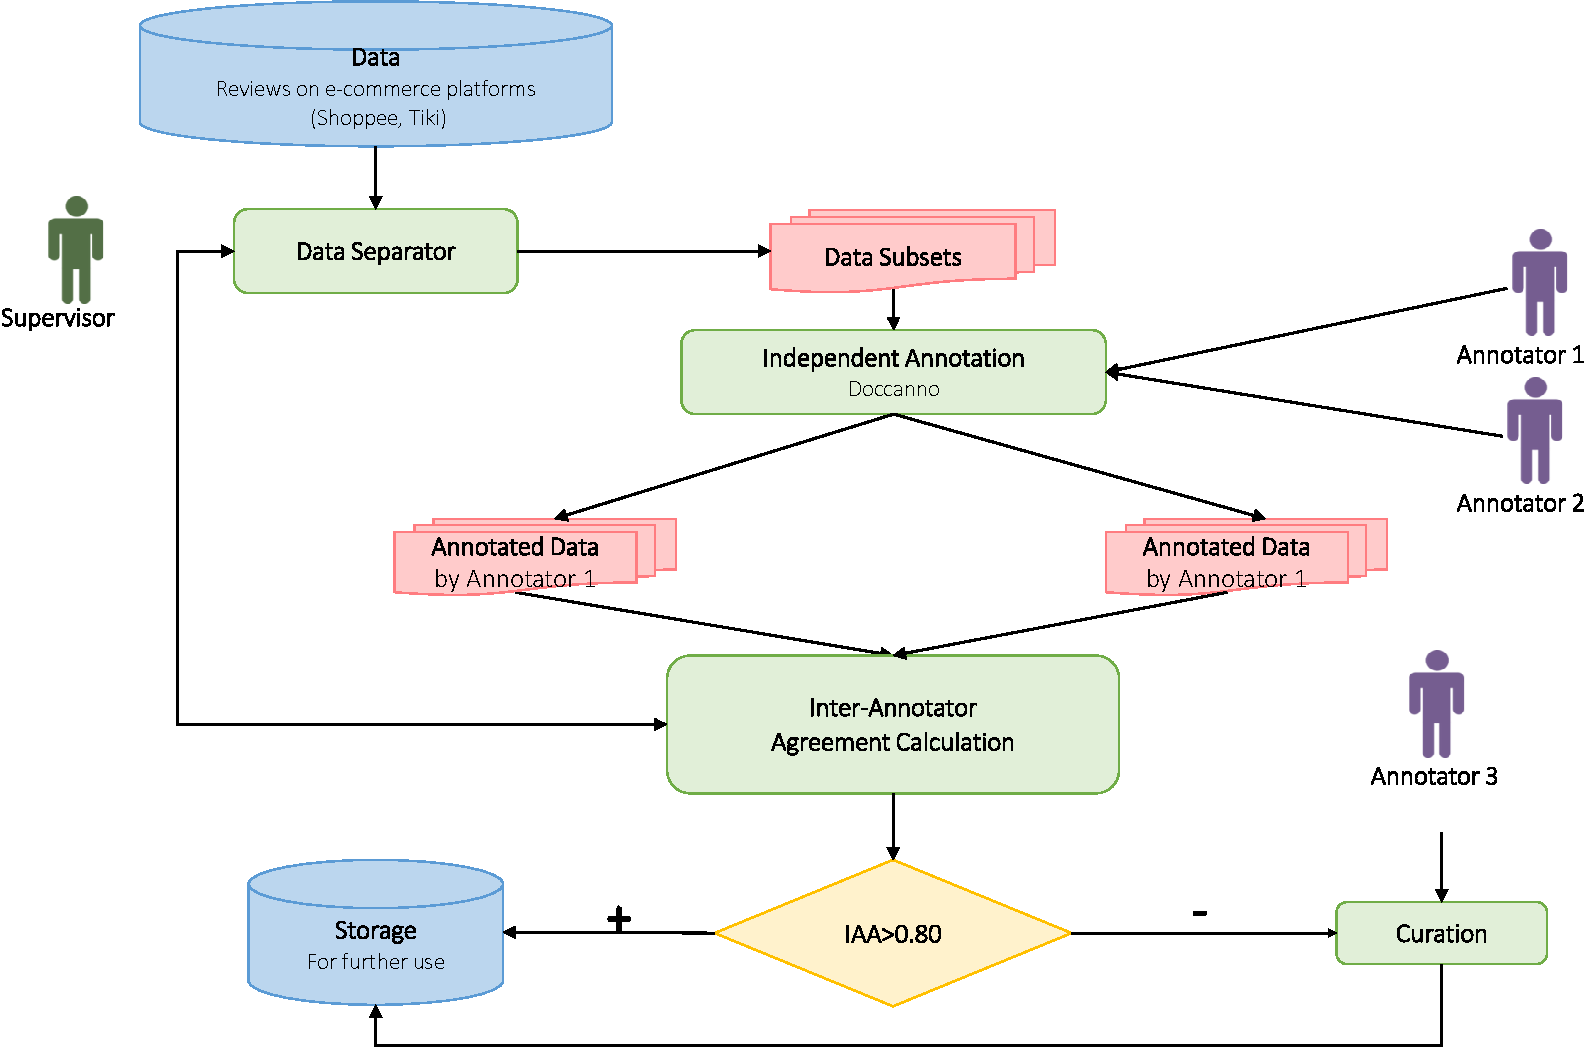
\includegraphics[width=\linewidth]{Chapter2/Figs/annotation.pdf}
	\caption{Data Annotation process}
	\label{fig:annotation}
\end{figure}

Data then separated in subsets, each of them was then evaluated and labeled by 2 annotators independently. Next, we measured the agreement between two annotators, if the result is too low (Inter-Annotator Agreement or IAA \(<\) 0.8), manually reviewing – process will be applied. The labeled data then stored as input for Pre-processing step. 

% -------------------------------------------------------------------
% Dataset Analysis
% -------------------------------------------------------------------
\section{Dataset Analysis}
\label{sec:data-analysis}
\paragraph{}
The statistics of Vietnamese E-commerce dataset (VECD) including Shopee and Tiki in two different domains:  Technology and Mother \& Baby are reported in figure 1 to 4. VECD consists of 3016 instances of Shopee Mother \& Baby, 2986 instances of Tiki , 3002 instances of Shopee Technology and 3236 instances of Tiki Technology, making up 12240 instances in total.

\begin{table}[h]
\centering
\begin{tabular}{|l|c|c|c|c|}
\hline
\multirow{2}{*}{}                                        & \multicolumn{2}{c|}{\textbf{Mother \& Baby}}           & \multicolumn{2}{c|}{\textbf{Technology}}                \\ \cline{2-5} 
                                                         & \textit{\textbf{Shopee}} & \textit{\textbf{Tiki}} & \textit{\textbf{Shopee}} & \textit{\textbf{Tiki}} \\ \hline
\multicolumn{1}{|c|}{\textbf{Total aspect}}              & 6                        & 6                      & 8                        & 8                      \\ \hline
\multicolumn{1}{|c|}{\textbf{Aspect count per sentence}} & 1.753234                 & 1.497347               & 2.087627                 & 1.746551               \\ \hline
\end{tabular}
\caption{The average number of aspects mentioned}
\end{table}

\begin{figure}[h]
	\centering
	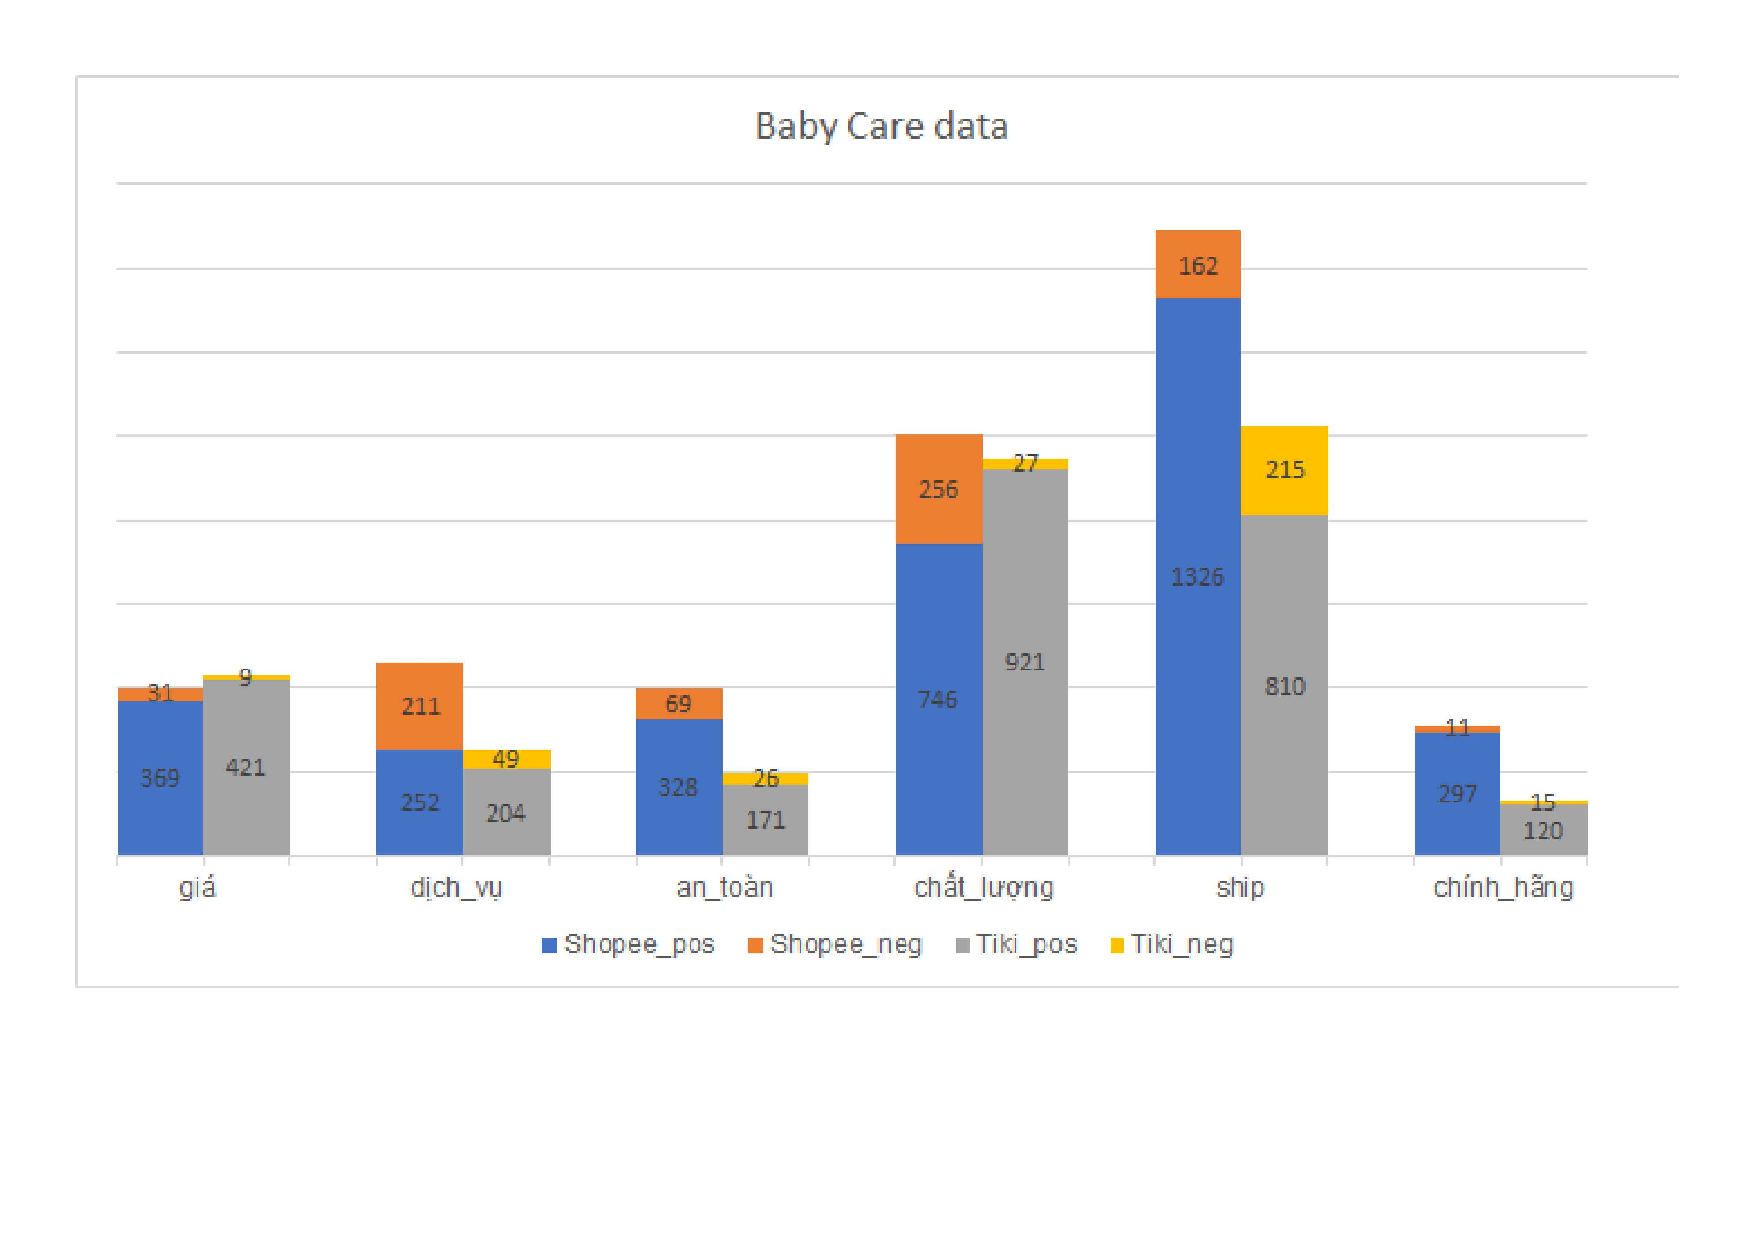
\includegraphics[width=\linewidth]{Chapter2/Figs/baby care.pdf}
	\caption{Mother \& Baby data statistics}
	\label{fig:baby}
\end{figure}

In Mother \& Baby domain, Shipping and Quality appear to be the most concerned aspects. Shopee has $1541$/$3216$ comments on Shipping and $773$/$3216$ comments on Quality, while in Tiki they are $972$/$2986$ and $1177$/$2986$ respectively. Authenticity only occasionally mentioned in Tiki's comments, just in $131$ cases while the others are mentioned in over $200$ comments, in both platforms, including Authenticity mentioned in Shopee.

Similarly, in Technology domain, Appearance is frequently mentioned in Shopee while it is Shipping in Tiki. More specifically $1064$ out of $3002$ comments on Shopee have information relating to products’ appearance, compared to $1021$ out of $3236$ comments on Tiki having information about Shipping. Price and Authenticity are the most imbalanced aspects, with only $4$ negative comments on Price and $12$ negative comments on Authenticity in Shopee while in Tiki the figures are $31$ and $24$, respectively. In Tiki, although the number of comments on Service, Hardware, Performance and Accessories is comparatively low, the data on these aspects are relatively balanced, with the difference below $16\%$.

\begin{figure}[]
	\centering
	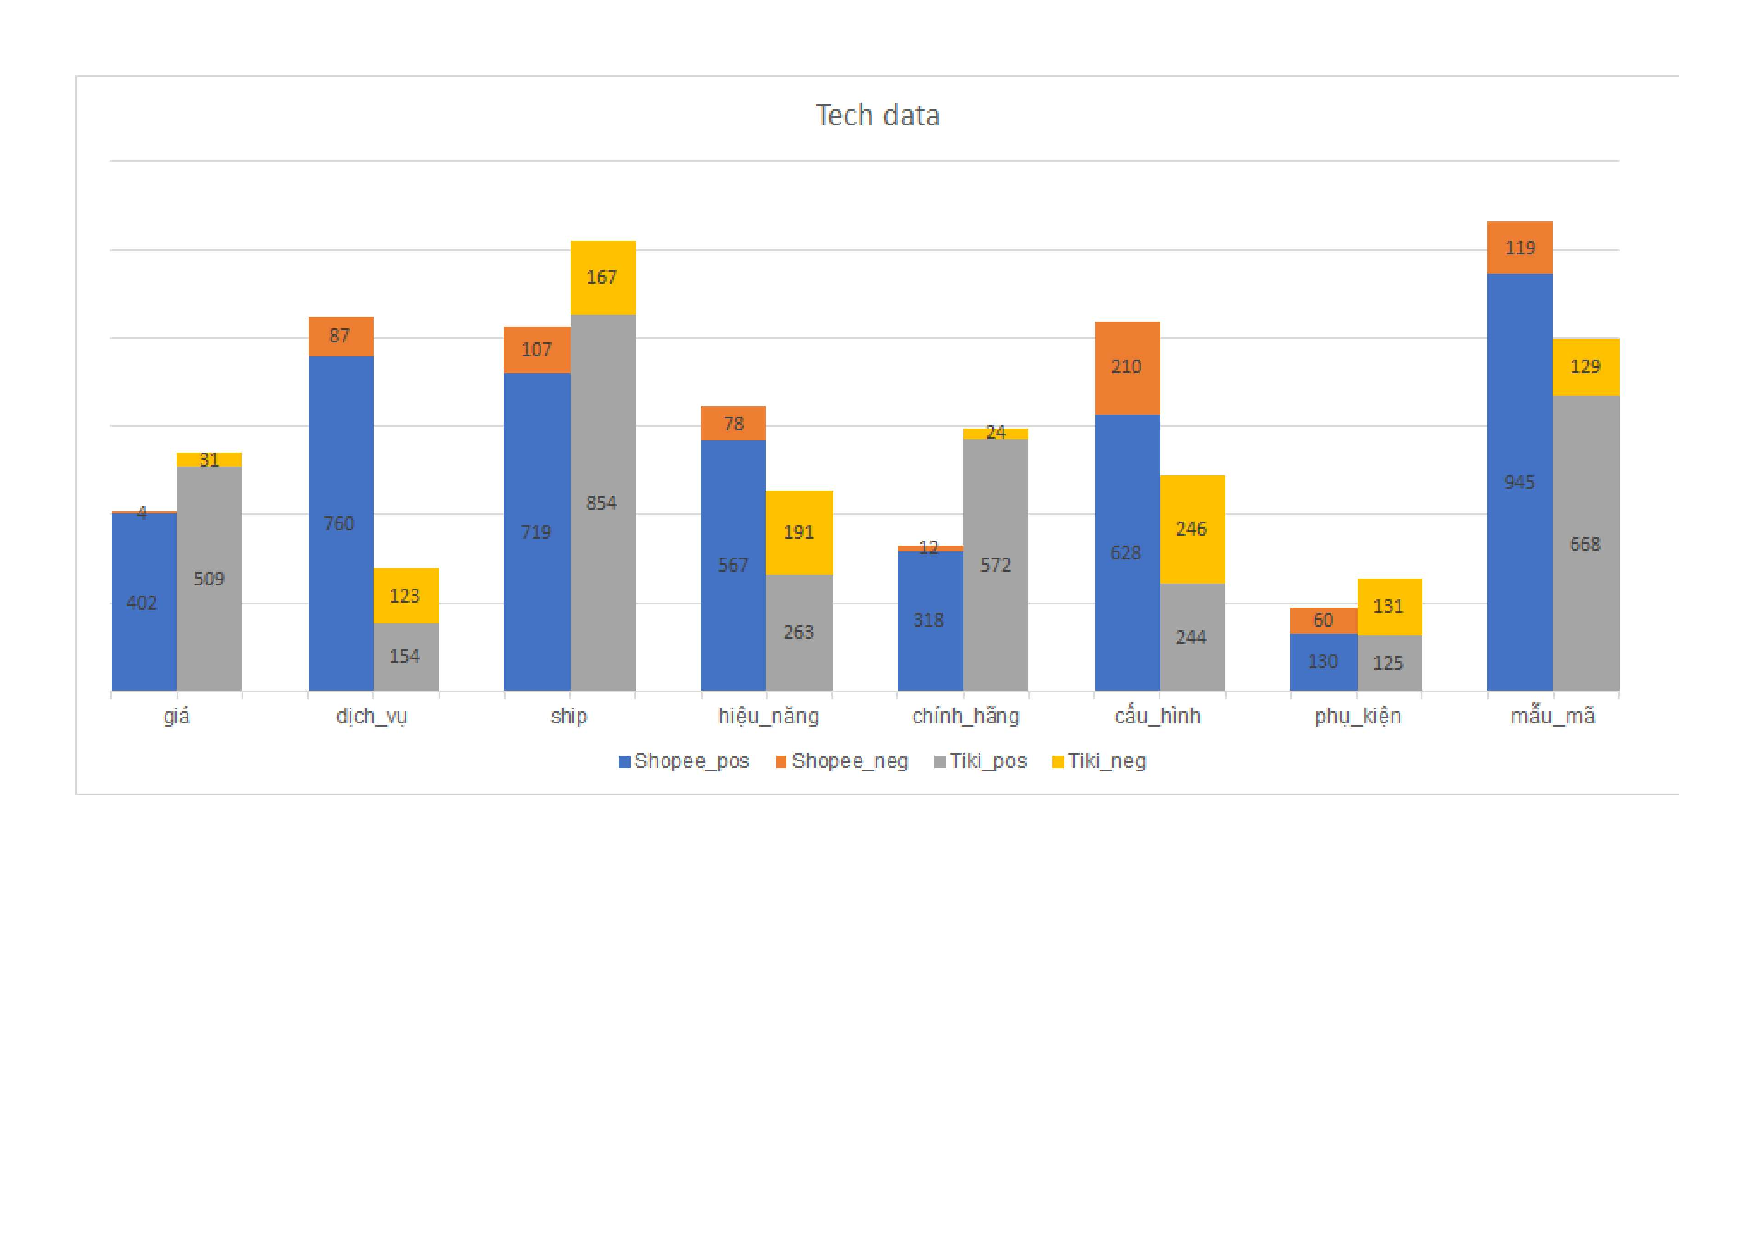
\includegraphics[width=\linewidth]{Chapter2/Figs/tech data.pdf}
	\caption{Technology data statistics}
	\label{fig:tech}
\end{figure}













% \include{Chapter6/chapter6}


% % List of publications
% \chapter*{List of Publications}
\addcontentsline{toc}{chapter}{List of Publications}

\begin{enumerate}[label={[Pub \arabic*]},leftmargin=3cm]

\item \underline{\textbf{Duy-Cat Can}}, Hoang-Quynh Le, Quang-Thuy Ha, and Nigel Collier. ``A Richer-but-Smarter Shortest Dependency Path with Attentive Augmentation for Relation Extraction.'' In \textit{The 2019 Annual Conference of the North American Chapter of the Association for Computational Linguistics: Human Language Technologies (NAACL-HTL)}, 2019, (In Press).

\item \underline{\textbf{Duy-Cat Can}}, Hoang-Quynh Le, and Quang-Thuy Ha. ``Improving Semantic Relation Extraction System with Compositional Dependency Unit on Enriched Shortest Dependency Path.'' In \textit{The 11th Asian Conference on Intelligent Information and Database Systems (ACIIDS)}, pp. 140-152, Springer, 2019.

\item Trang M. Nguyen, Van-Lien Tran, \underline{\textbf{Duy-Cat Can}}, Quang-Thuy Ha, Ly T. Vu, and Eng-Siong Chng. ``QASA: Advanced Document Retriever for Open-Domain Question Answering by Learning to Rank Question-Aware Self-Attentive Document Representations.'' In \textit{Proceedings of the 3rd International Conference on Machine Learning and Soft Computing}, pp. 221-225. ACM, 2019.

\item \underline{\textbf{Duy-Cat Can}}, Thi-Nga Ho, and Eng-Siong Chng. ``A hybrid deep learning architecture for sentence unit detection.'' In \textit{Proceedings of the 2018 International Conference on Asian Language Processing (IALP)}, pp. 129-132. IEEE, 2018.

\item Thi-Nga Ho, \underline{\textbf{Duy-Cat Can}}, and Eng-Siong Chng. ``An investigation of word embeddings with deep bidirectional lstm for sentence unit detection in automatic speech transcription.'' In \textit{Proceedings of the International Conference on Asian Language Processing (IALP)}, pp. 139-142. IEEE, 2018.

\item Hoang-Quynh Le, \underline{\textbf{Duy-Cat Can}}, Sinh T. Vu, Thanh Hai Dang, Mohammad Taher Pilehvar, and Nigel Collier. ``Large-scale exploration of neural relation classification architectures.'' In \textit{Proceedings of the 2018 Conference on Empirical Methods in Natural Language Processing (EMNLP)}, pp. 2266-2277. 2018.

\end{enumerate}

%--------------------------------------------- 
% References
%---------------------------------------------
\bibliographystyle{IEEEtranSN}
\renewcommand\bibname{References}
\addcontentsline{toc}{chapter}{References}
\bibliography{references} % Path to your references.bib file

%--------------------------------------------- 
% Appendix
%---------------------------------------------
\appendix
% \chapter{List of Publications}
Appendix A

\end{document}
